\chapter*{CI-2-3 track}
\addcontentsline{toc}{chapter}{CI-2-3 track}
\label{ci-track}

\begin{figure}[h!]
\centering
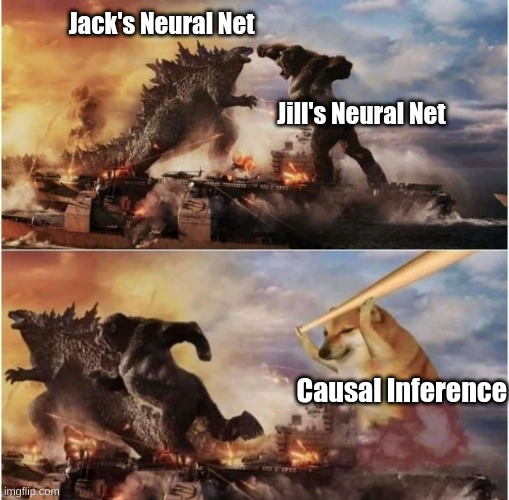
\includegraphics[width=5in]
{godzilla-kk-doge-nn-ci.jpg}
\caption{CI meme}
\label{fig-godzilla-kk-doge}
\end{figure}

\begin{figure}[h!]
\centering
\includegraphics[width=6in]
{pearl-ijcai-2022.jpg}
\caption{Slide from Pearl talk at IJCAI-2022. 
Putting the joking 
of Fig.\ref{fig-godzilla-kk-doge} aside, 
let me emphasize that CI advocates 
are not trying to vanish
NNs from AI. To us,
NNs and bnets
are different tools, like 
hammer and saw. 
We believe AI should use both tools.
For those
who are trying to do
CI using a NN instead of a
bnet, it looks to me like you are
trying to use a hammer
to cut wood. Why don't you cut with 
a saw instead?
As Pearl says in this slide,
CI elevates Data Science
from Deep Learning (data-fitting) to 
Deep Understanding. }
\label{fig-deep-understanding}
\end{figure}


As discussed in Chapter \ref{ch-counterf},
Judea Pearl has proposed 3 rungs
of Causal Inference (CI).
This book covers all 3 rungs.

Confusingly,
it has become common to use the term
CI to refer to only the highest
2 rungs of the CI hierarchy; i.e,
rung 2 (do operations)
and rung 3 (imagining/counterfactual thinking).
Also confusingly, rung 1
uses causal diagrams and
is often referred to as ``inference",
so it could reasonably have been defined as the whole
of CI, but Pearl has defined
the CI hierarchy to include two more rungs.
To patch over this linguistic confusion,
I sometimes refer to rung 1 as ``prediction",
or as ``predictive inference"
instead of calling it merely ``inference".
Also, when I want to be precise,
I use the term ``CI-2-3" to
refer to CI restricted to only rungs 2 and 3.


Here is a subset of chapters
that I call
the CI-2-3 track,
that are devoted mostly to rungs 2 and 3.


\begin{enumerate}
\item \nameref{ch-bdoor}
\item \nameref{ch-berkson}
\item \nameref{ch-counterf}
\item \nameref{ch-dec-2-3}
\item \nameref{ch-did}
\item \nameref{ch-do-calc}
\item \nameref{ch-do-calc-proofs}
\item \nameref{ch-dsep}
\item \nameref{ch-dsep-lden}
\item \nameref{ch-fwl-theo}
\item \nameref{ch-fdoor}
\item \nameref{ch-g-formula}
\item \nameref{ch-good-causal-fit}
\item \nameref{ch-granger-c}
\item \nameref{ch-inst-ineq}
\item \nameref{ch-instrumental}
\item \nameref{ch-late}
\item \nameref{ch-mediation}
\item \nameref{ch-meta-learners}
\item \nameref{ch-modi-treat}
\item \nameref{ch-personalized}
\item \nameref{ch-personalized-test}
\item \nameref{ch-pot-out}
\item \nameref{ch-reg-dis}
\item \nameref{ch-sb-removal}
\item \nameref{ch-simpson}
\item \nameref{ch-survival}
\item \nameref{ch-syn-con}
\item \nameref{ch-targeted-est}
\item \nameref{ch-transport}
\item \nameref{ch-uplift}
\end{enumerate}
